%%%%%%%%%%%%%%%%%%%%%%%%%%%%%%%%%%%%%%%%%%%%%%%%%%%%%%%
% use this declaration for a draft  version of your IS
\documentclass[10pt,palatino,code,picins,kaukecopyright,openright,woolshort,dropcaps,verbatim,index,euler]{woosterthesis}
%\documentclass[10pt,code,picins,kaukecopyright,openright,woolshort,dropcaps,verbatim,euler,index,colophon,blacklinks,twoside]{woosterthesis}
% note that you can specify the woosterchicago option to use Chicago citation style and achemso to use the American Chemical Society citation format
%
%%%%%%%%%%%%%%%%%%%%%%%%%%%%%%%%%%%%%%%%%%%%%%%%%%%%%%%
%
% use this declaration for the print version of your IS
%\documentclass[12pt,code,palatino,picins,blacklinks,kaukecopyright,openright,twoside]{woosterthesis} % probably what most students would use
%
%%%%%%%%%%%%%%%%%%%%%%%%%%%%%%%%%%%%%%%%%%%%%%%%%%%%%%%
%
% use this declaration for the PDF version of your IS
%\documentclass[12pt,code,palatino,picins,kaukecopyright,openright,twoside]{woosterthesis}
%
%%%%%%%%%%%%%%%%%%%%%%%%%%%%%%%%%%%%%%%%%%%%%%%%%%%%%%%

\usepackage{wasysym}

%%%%%%%%%%%%%%%%%%%%%%%%%%%%%%%%%%%%%%%%%%%%%%%%%%%%%%%%%%%%%%%%%%%%%%%%%%%%%%%%%%%%%%%%%%%%%%
%
%                                                       Packages
%
% Do not add any other packages without consulting with Dr. Breitenbucher as they may break the functionality of the class.
%
%%%%%%%%%%%%%%%%%%%%%%%%%%%%%%%%%%%%%%%%%%%%%%%%%%%%%%%%%%%%%%%%%%%%%%%%%%%%%%%%%%%%%%%%%%%%%%

\ifxetex%
	\defaultfontfeatures{Mapping=tex-text}%
		\setmainfont[Numbers=OldStyle,BoldFont={* Semibold}]{Adobe Garamond Pro}% select the body font other choices would be Baskerville, Optima Regular, Didot, Georgia, Cochin
                      \setmathrm{Adobe Garamond Pro}
                      \setmathfont[Digits,Latin]{Adobe Garamond Pro}
		\setsansfont[Scale=.87,Fractions=On,Numbers=Lining]{Myriad Pro}% select the sans serif font other choices would be Skia, Arial, Helvetica, Helvetica Neue
%		\setmonofont[Scale=.88,Fractions=On]{Prestige Elite Std Bold}% set the mono font other choices would be Courier, Monaco, American Typewriter
	           \setmonofont[Scale=.9]{Courier Std}%
%	    \setromanfont[Fractions=On,Numbers=OldStyle, BoldFont={Warnock Pro Semibold}]{Warnock Pro}%
%	    \setsansfont[Scale=.95,Fractions=On,Numbers=Lining]{Myriad Pro}%
%	    \setmonofont[Scale=.91,Fractions=On]{Courier Std Medium}%
%	    \setmonofont[Scale=.88,Fractions=On]{American Typewriter}%
%		\setmonofont[Scale=.94,Fractions=On]{Prestige Elite Std Bold}
%    		\setromanfont[Fractions=On,Numbers=OldStyle]{Minion Pro}
 %    	\setsansfont[Scale=.9,Fractions=On,Numbers=Lining]{Myriad Pro}
%     	\setmonofont[Scale=.93,Fractions=On]{Courier Std Medium}
%     	\setromanfont[Fractions=On,Numbers=OldStyle]{Minion Pro}
%     	\setsansfont[Scale=.85,Fractions=On,Numbers=Lining]{News Gothic Std}
%    		\setmonofont[Scale=.93,Fractions=On]{Prestige Elite Std}
%		\setromanfont[Fractions=On,Numbers=OldStyle]{Minion Pro}
%		\setsansfont[Scale=.9,Fractions=On,Numbers=Lining]{Bell Gothic Std Bold}
%		\setmonofont[Scale=.95,Fractions=On]{Prestige Elite Std Bold}
\fi

%%%%%%%%%%%%%%%%%%%%%%%%%%%%%%%%%%%%%%%%%%%%%%%%%%%%%%%%%%%%%%%%%%%%%%%%%%%%%%%%%%%%%%%%%%%%%%
%
%                                                       Personal Commands
%                                                                    
% There will be certain commands that you use frequently in the thesis. You can give these
% commands new names which are easier for you to remember. You can also combine several
% commands into a new command of your own. See The LaTeX Companion or Guide to LaTeX for
% examples on defining your own commands. These are commands that I defined to cut down on typing.
%
%%%%%%%%%%%%%%%%%%%%%%%%%%%%%%%%%%%%%%%%%%%%%%%%%%%%%%%%%%%%%%%%%%%%%%%%%%%%%%%%%%%%%%%%%%%%%%

\newcommand{\fl}{\ell}
\newcommand{\lt}{\LaTeX\ }
\newcommand{\msw}{Word\texttrademark\ }
\newcommand{\xt}{\ifthenelse{\boolean{xetex}}{\XeTeX\ }{XeTeX} }
%\newcommand{\Cl}{\ensuremath{\textup{C}_\fl}}
%\newcommand{\bCl}{C$_{\ell}$}
%\newcommand{\Al}{\ensuremath{\textup{A}_\fl}}
%\newcommand{\msum}{{(m_1+\cdots+m_\ell)}}
%\newcommand{\Nsum}{{(N_1+\cdots+N_\ell)}}
%\newcommand{\ysum}{{(y_1+\cdots+y_\ell)}}
%\newcommand{\Nsub}{{N_1+\cdots+N_\ell}}
%\newcommand{\ysub}{{y_1+\cdots+y_\ell}}
%\newcommand{\xsub}{{x_1+\cdots+x_\ell}}
%\newcommand{\ysqsum}{{y_1^2+\cdots +y_{\fl}^2}}
%\newcommand{\msqsum}{{m_1^2+\cdots +m_{\fl}^2}}
%\newcommand{\ratio}{\left(\frac{\beta}{\alpha}\right)}
%\newcommand{\LT}{\ensuremath{\LaTeX{}}}

%%%%%%%%%%%%%%%%%%%%%%%%%%%%%%%%%%%%%%%%%%%%%%%%%%%%%%%%%%%%%%%%%%%%%%%%%%%%%%%%%%%%%%%%%%%%%%
% These commands have one argument and are entered as \commandname{argument}.
%%%%%%%%%%%%%%%%%%%%%%%%%%%%%%%%%%%%%%%%%%%%%%%%%%%%%%%%%%%%%%%%%%%%%%%%%%%%%%%%%%%%%%%%%%%%%%

%\newcommand{\bd}[1]{\textbf{#1}}
\newcommand{\mbd}[1]{{\mathbf{#1}}}
%\newcommand{\abs}[1]{\vert{#1}\vert}
\newcommand{\bvec}[1]{{\mbd{#1}}}
%\newcommand{\lvec}[1]{\abs{\bvec{#1}}}
%\newcommand{\nesmallprod}[1]{\prod_{\substack{#1=1\\
%#1\neq p}}^{\fl}}
%\newcommand{\esec}[1]{e_{2}({#1}_1,\ldots ,{#1}_\fl)}
%\newcommand{\smallprod}[1]{\prod_{#1=1}^{\fl}}
%\newcommand{\incsum}[1]{{#1}_2+2{#1}_3+\cdots +(\fl -1){#1}_\fl}
%\newcommand{\binomsum}[1]{\binom{{#1}_1}{2}+\cdots +\binom{{#1}_\fl}{2}}
%\newcommand{\imultsum}[1]{\multsum{{#1}_k\ge 0}{k=1,\ldots ,\fl}}
%\newcommand{\diagsum}[1]{\sum _{\substack{{#1}_k\ge 0\\
%k=1, \ldots ,\fl\\
%\lvec{#1}=m}}}
%\newcommand{\Mb}[1][\fl]{\ensuremath{\textup{\bd{M}}_b^{(#1)}}}
%\newcommand{\HLV}[1]{\ensuremath{\textup{\bd{H}}_{#1}}}
%\newcommand{\Rq}[1][p]{\ensuremath{\textup{R}_q^{(#1)}}}
\newcommand{\degree}[1]{\ensuremath{#1^{\circ}}}
\newcommand{\ip}[1]{\texttt{#1}\index{packages!#1}}
\newcommand{\ic}[1]{\texttt{$\backslash$#1}\index{commands!#1}}
\newcommand{\ie}[1]{#1\index{#1}}

%%%%%%%%%%%%%%%%%%%%%%%%%%%%%%%%%%%%%%%%%%%%%%%%%%%%%%%%%%%%%%%%%%%%%%%%%%%%%%%%%%%%%%%%%%%%%%
% These commands have 2 or more arguments some with default values for the first argument. You
% can learn a lot about constructing complicated equations by studying the commands in this %section.
%%%%%%%%%%%%%%%%%%%%%%%%%%%%%%%%%%%%%%%%%%%%%%%%%%%%%%%%%%%%%%%%%%%%%%%%%%%%%%%%%%%%%%%%%%%%%%

%\newcommand{\qbinom}[2]{\ensuremath{\left[{#1}\atop{#2}\right]_q}}
%\newcommand{\sqprod}[2]{\prod_{#1,#2=1}^{\fl}}
%\newcommand{\triprod}[2]{\prod_{1\le #1<#2\le \fl}}
%\newcommand{\nesqprod}[2]{\prod_{\substack{#1,#2=1\\
%#1,#2\neq p}}^{\fl}}
%\newcommand{\netriprod}[2]{\prod_{\substack{1\le #1<#2\le \fl\\
%#1,#2\neq p}}}
\newcommand{\qrfac}[3][\ ]{\left({#2}\right)_{#3}^{#1}}
%\newcommand{\multsum}[2]{\sum_{\substack{{#1}\\
%\\
%{#2}}}}
%\newcommand{\fmultsum}[2][N]{\multsum{0\le {{#2}_k}\le {{#1}_k}}{k=1,\ldots ,\fl}}
%\newcommand{\pq}[2]{\ _{#1}\varphi_{#2}}
%\newcommand{\mess}[2][y_k]{\frac{\qrfac{\alpha x_k}{#2}\qrfac{qx_k\beta^{-1}}{#2}}{\qrfac{\beta x_k}{#1}
%\qrfac{qx_k\alpha^{-1}}{#1}}}
%\newcommand{\MG}[7][\fl]{\ensuremath{\left[\textup{MG}\right]_{#2}^{(#1)}{#3}q;{#4};{#5}^{#6}{#7}}}

%%%%%%%%%%%%%%%%%%%%%%%%%%%%%%%%%%%%%%%%%%%%%%%%%%%%%%%%%%%%%%%%%%%%%%%%%%%%%%%%%%%%%%%%%%%%%%
% These commands define new environments
%%%%%%%%%%%%%%%%%%%%%%%%%%%%%%%%%%%%%%%%%%%%%%%%%%%%%%%%%%%%%%%%%%%%%%%%%%%%%%%%%%%%%%%%%%%%%%

\newcounter{unnumft}
\setcounter{unnumft}{0}
\newenvironment{unnumft}[2]{\renewcommand{\thefootnote}{}\footnote{#1}\footnote{#2}} {\addtocounter{footnote}{-2}}
\newenvironment{wooexample}{\small
\begin{singlespace}
\begin{example}}{\end{example}
\end{singlespace}}

\graphicspath{{./figures/}}% for setting where to look for figures
\citestyle{wooster}% change the style of citations. Math and CS people should leave this alone.






%%%%%%%%%%%%%%%%%%%%%%%%%%%%%%%%%%%%%%%%%%%%%%%%%%%%%%%%%%%%%%%%%%%%%%%%%%%%%%%%%%%%%%%%%%%%%%
%
% This is where one would tell \LaTeX{} how to format Theorems, Definitions, etc. and also
% indicate the environment names. You need the amsthm package (loaded in the woosterthesis %class) in order for these commands to work.
%
%%%%%%%%%%%%%%%%%%%%%%%%%%%%%%%%%%%%%%%%%%%%%%%%%%%%%%%%%%%%%%%%%%%%%%%%%%%%%%%%%%%%%%%%%%%%%%

% an example of defining your own theoremstyle
%\newtheoremstyle{break}% name
%  {\topsep}%      Space above
%  {\topsep}%      Space below
%  {\itshape}%         Body font
%  {}%         Indent amount (empty = no indent, \parindent = para indent)
%  {\bfseries}% Thm head font
%  {.}%        Punctuation after thm head
%  {\newline}%     Space after thm head: " " = normal interword space;
%        %       \newline = linebreak
%  {}%         Thm head spec (can be left empty, meaning `normal')
\newtheoremstyle{scthm}{\topsep}{\topsep}{\itshape}{}{\bfseries\scshape}{}{ }{}% small cap font for the heading
\newtheoremstyle{itdefn}{\topsep}{\topsep}{\itshape}{}{\bfseries}{.}{ }{}% italic definitions
\newtheoremstyle{scdefn}{\topsep}{\topsep}{\itshape}{}{}{}{ }{\thmname{\textbf{#1}}\thmnumber{ \textbf{#2}}\thmnote{ \scshape #3:}}% small cap headings and italic text.

\theoremstyle{break}% this theoremstyle will put the text of the theorem on a new line.
\newtheorem{thm}{Theorem}[chapter]%number theorems within chapters 
%\newtheorem{cor}[thm]{Corollary}%by using [thm] we are numbering these environments with the theorems.
\newtheorem{cor}{Corollary}[chapter]%number corollaries within chapters .
%\newtheorem{lem}[thm]{Lemma}
\newtheorem{lem}{Lemma}[chapter]
%\newtheorem{prop}[thm]{Proposition}
\newtheorem{prop}{Proposition}[chapter]

\theoremstyle{scdefn}
%\newtheorem{defn}[thm]{Definition}
\newtheorem{defn}{Definition}[chapter]
\theoremstyle{remark}
%\newtheorem{rem}[thm]{Remark}
\newtheorem{rem}{Remark}[chapter]
\renewcommand{\therem}{}
%\newtheorem{ex}[thm]{Example}
\newtheorem{ex}{Example}[chapter]

\theoremstyle{plain}
%\newtheorem{note}[thm]{Notation}
\newtheorem{note}{Notation}[chapter]
\renewcommand{\thenote}{}
%\newtheorem{nts}[thm]{Note to self}%use to remind yourself of things yet to do
\newtheorem{nts}{Note to self}[chapter]
\renewcommand{\thents}{}
%\newtheorem{terminology}[thm]{Terminology}
\newtheorem{terminology}{Terminology}[chapter]
\renewcommand{\theterminology}{}

\theoremstyle{itdefn}
\newtheorem{bdefn}{Definition}[chapter]
\newsavebox{\fmbox} 
\newenvironment{boxeddefn}[2] 
{\begin{lrbox}{\fmbox}\begin{minipage}{0.9 \linewidth }\begin{singlespace}\begin{bdefn}[{#1}]\label{#2}\vspace{0.2cm}} 
{\end{bdefn}\end{singlespace}\end{minipage}\end{lrbox}\fbox{\usebox{\fmbox}}}

\setcounter{secnumdepth}{5}% controls the numbering of sections
\setcounter{tocdepth}{6}% controls the number of levels in the Contents

\title{Algorithmic Music Composition}
\thesistype{Independent Study Thesis}
\author{Thomas Matlak}
\degreetoobtain{B.A.}
\presentschool{The College of Wooster}
\academicprogram{Departments of Computer Science and Mathematics}
\gradyear{2018}
\advisor{Nathan Sommer (Computer Science)}
\secondadvisor{Nathan Fox (Mathematics)}
%\reader{Reader}
\copyrighted   
%\copyrightdate{}                  
\makeindex % comment this line if you do not have an index

\begin{document}

%%%%%%%%%%%%%%%%%%%%%%%%%%%%%%%%%%%%%%%%%%%%%%%%%%%%%%%
%
%  The front matter includes acknowledgments, dedications, vitas, list of tables, list of figures,
%  copyright, abstract, title page, and contents.
%
%%%%%%%%%%%%%%%%%%%%%%%%%%%%%%%%%%%%%%%%%%%%%%%%%%%%%%%

\frontmatter
\maketitle
\ClearShipoutPicture
\clearpage\thispagestyle{empty}\null\clearpage
\disscopyright 

% Abstract

\begin{abstract} \label{abstract}
Algorithmic music composition is a popular area of research in computer aided music; it is the application of computer algorithms to create music.
One subtopic of this area is the automated creation of pleasing melodies.
This paper explores two machine learning approaches to algorithmically creating melodies: Markov chains and genetic algorithms.
Markov chains can generate a rough imitation of the corpus of music upon which they are based.
Though Markov chains can generate a rough approximation of a musical style, we want to refine the music to bring it closer to the desired target style.
To accomplish this we use genetic algorithms to take an initial population of melodies and tweak and remix them to create better melodies.
Genetic algorithms have been used extensively in previous research, but this paper proposes the use of a long short-term memory artificial neural network to act as a surrogate fitness function, rather than defining a set of rules for good music and penalties for breaking those rules.
\end{abstract}

% Dedications

\dedication{This work is dedicated to the future generations of Wooster students.}

% Acknowledgments

\begin{acknowl}  

\end{acknowl}

% Vita

\begin{vita} 
% You talk about yourself and how you got to where you are now. There is a structured form for the Vita that can be used if you want, but I don't encourage it.

%%%%%%%%%%%%%%%%%%%%%%%%%%%%%%%%%%%%%%%%%%%%%%%%%%%%%%%
%
%  The list below is for a thesis that requires a more structured Vita such as a masters or Ph.D.
%
%%%%%%%%%%%%%%%%%%%%%%%%%%%%%%%%%%%%%%%%%%%%%%%%%%%%%%%

%\begin{datelist}
%\item[April 6, 1970]Born-Wooster, Ohio
%\item[August 11, 1990]Chosen to present an undergraduate paper at the 75th meeting of the MAA, Columbus, Ohio
%\item[August 1990--August 1991]President Wooster Student Chapter of the MAA, The College of Wooster, Wooster, Ohio
%\item[August 1991--May 1992]Secretary Wooster Student Chapter of the MAA, The College of Wooster, Wooster, Ohio
%\item[1992]\emph{Phi Beta Kappa} (on junior standing), The College of Wooster, Wooster, Ohio
%\item[1992]Elizabeth Sidwell Wagner Prize in Mathematics, The College of Wooster
%\item[1992]William H. Wilson Prize in Mathematics, The College of Wooster
%\item[May 11, 1992]B.A., Mathematics, The College of Wooster
%\item[1997]Finalist for Graduate Teaching Award, The Ohio State University, Columbus, Ohio
%\item[June 21-25, 1998]Participant in the AMS-IMS-SIAM Summer Research Conferences: q-Series, Combinatorics, and Computer Algebra, Mt. Holyoke, Massachusetts
%\item[October 1998--October 1999]Graduate student representative to The Ohio State University Department of Mathematics Graduate Studies Committee, Columbus, Ohio
%\item[January 1999]q-series seminar address, The Ohio State University, Columbus, Ohio
%\item[2000]Finalist for Departmental Teaching Award, The Ohio State University, Columbus, Ohio
%\item[2000]Nominated for Graduate Teaching Award, The Ohio State University, Columbus, Ohio
%\item[April 2000]Invited colloquium talk at The College of Wooster, Wooster, Ohio
%\item[1992-- present]Graduate Teaching and Research Associate, The Ohio State University
%\end{datelist}
%
%%%This is for any publications you might have.%%%%%

%\begin{publist}  
%\pubitem{\quad}
%\pubitem{\quad}
%\end{publist}

\begin{fieldsstudy} 
    \majorfield{Computer Science and Mathematics}
	\minorfield{Music}
%    \specialization{Algorithmic Compositions}
    %\begin{studieslist}
   %\studyitem{Abstract Algebra}{Hampton}
   %\end{studieslist}
  \end{fieldsstudy}
\end{vita}

%%%%%%%%%%%%%%%%%%%%%%%%%%%%%%%%%%%%%%%%%%%%%%%%%%%%%%%
%
%  We now create the contents page and if necessary the list of figures and list of tables.
%
%%%%%%%%%%%%%%%%%%%%%%%%%%%%%%%%%%%%%%%%%%%%%%%%%%%%%%%


\cleardoublepage
\phantomsection
\addcontentsline{toc}{chapter}{Contents}

\tableofcontents
\listoffigures %Use if you have a list of figures.
\listoftables%Use if you have a list of tables.
% \lstlistoflistings% Use if you are using the code option

%%%%%%%%%%%%%%%%%%%%%%%%%%%%%%%%%%%%%%%%%%%%%%%%%%%%%%%

% \input{chapters/preface} % most theses do not have a preface so this should be commented

%%%%%%%%%%%%%%%%%%%%%%%%%%%%%%%%%%%%%%%%%%%%%%%%%%%%%%%
\mainmatter

% Thesis chapters, each in a separate file

%!TEX root = ../username.tex
\chapter{Background} \label{bg}

This section contains the background information necessary to understand the project.

\section[Markov Chains]{Markov Chains} \label{bg:markov}

\subsection{Definition} \label{bg:markov:definitions}

A Markov Chain is a type of discrete-time stochastic process, which means a Markov Chain is a sequence of random variables $\boldsymbol{X} = \{X_{n} | n \in I\}$ for some index set $I$.
Additionally, Markov Chains have the special property that they depend only on the immediate past state(s).
That is, for a first-order Markov Chain at time $n$, $$P(X_{n} = j \mid X_{0} = i_{0}, \ldots, X_{n - 1} = i_{i - 1}) = P(X_{n} = j \mid X_{n - 1} = i_{n - 1})$$ for a particular possible outcome $j$ of $X_{n}$ \cite{nierhaus_algorithmic_2009}.

This idea can also extend to higher-order Markov Chains.
A higher-order Markov process considers more than the single most recent state to determine the next state.
An $n$th order Markov Chain uses the previous $n$ states as the input to find the next state.

\subsection{Representations} \label{bg:markov:representations}

We can think of a Markov Chain as a directed graph, where each state is a node, each edge is a transition between states, and the probabilities of transitioning between states are represented by the edge weights.
See Figure \ref{fig:markovGraph} for a visual representation of this idea.

\begin{figure}[h]
	\centering
	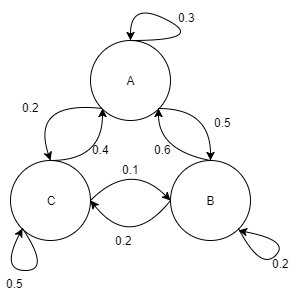
\includegraphics[]{figures/markovGraph.png} % TODO: Make a better diagram
	\caption{A Markov Chain represented as a graph.}
	\label{fig:markovGraph}
\end{figure}

When implementing a Markov Chain, however, it is perhaps easier to represent a is as an $(n + 1)$ dimensional array, where $n$ is the order of the Markov Chain.
See Figure \ref{fig:markovMatrix} for an example of the same Markov Chain as in Figure \ref{fig:markovGraph} in matrix form.

\begin{figure}[h]
	\centering
	\begin{tabular}{c | c c c}
		& $A_{1}$ & $B_{1}$ & $C_{1}$\\
		\hline
		$A_{0}$ & $0.3$ & $0.5$ & $0.2$\\
		$B_{0}$ & $0.6$ & $0.2$ & $0.2$\\
		$C_{0}$ & $0.4$ & $0.1$ & $0.5$
	\end{tabular}
	\caption{A Markov Chain represented as a transition matrix.}
	\label{fig:markovMatrix}
\end{figure}

\subsection{Limitations} \label{bg:markov:limitations}

A major limitation of Markov Chains is their inability to generate truly novel output.
In order for some state to appear, a transition to that state from the previous state must appear in the source.
Additionally, lower-order chains may produce nonsensical output, while a chain of sufficiently high order will exactly copy the source.
Another limitation is that the process may get stuck in a local loop.
This may happen when the chain proceeds to a state which only transitions to itself, or transitions to a set of states that only transition to each other.

%!TEX root = ../username.tex
\chapter{Mathematics In Music} \label{mathinmusic}

\section{The Harmonic Series} \label{mathinmusic:harmonic}

An important concept for pitch sounds is the harmonic series.
Pitched sounds have a fundamental frequency from which an overtone series is produced.
Overtones are any frequencies higher than the fundamental frequency.
The harmonic series is a restricted subset of the overtone series consisting of the integer multiples of the fundamental frequency.
For example, consider the open A string of a cello which is pitched as an A3.
In other words it has a fundamental frequency of $220$ Hz.
Doubling this frequency gives $440$ Hz, or an octave above the fundamental frequency.
Tripling the frequency gives $660$ Hz, which is an E5.
This continues, so multiplying by $4$ gives a frequency two octaves above the fundamental, multiplying by $5$ produces a C$\sharp$6, multiplying by $6$ gives an E6, multiplying by $7$ gives a G6, and multiplying by $8$ gives an A6, three octaves above the fundamental frequency.
We could go on, and eventually the frequencies would pass out of the human hearing range (approximately $20,000$ Hz).

The presence of the overtone series, and in particular the harmonic series is what makes a sound pitched.
Percussive sounds such as hitting a drum or dropping a brick do produce pressure in the air, but the oscillations of the pressure are not regular, and so do not produce any pitched frequencies.

\begin{figure}
	\centering
	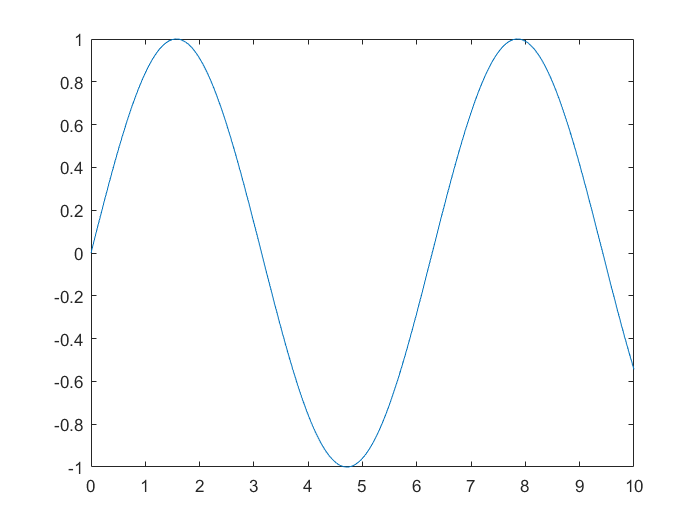
\includegraphics[width=\textwidth]{../figures/sinWave.png}
	\caption{A pure sin wave}
	\label{fig:sin}
\end{figure}

\begin{figure}
	\centering
	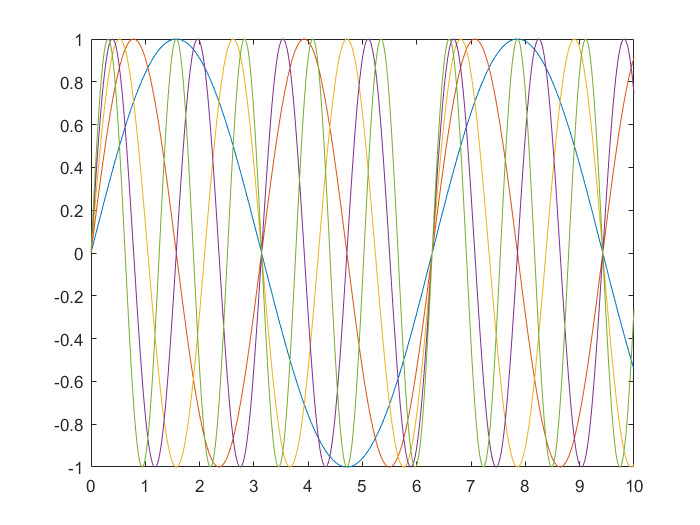
\includegraphics[width=\textwidth]{../figures/harmonicSinWaves.png}
	\caption{The first five harmonic frequencies of a sin wave.}
	\label{fig:harmonics}
\end{figure}

\begin{figure}
	\centering
	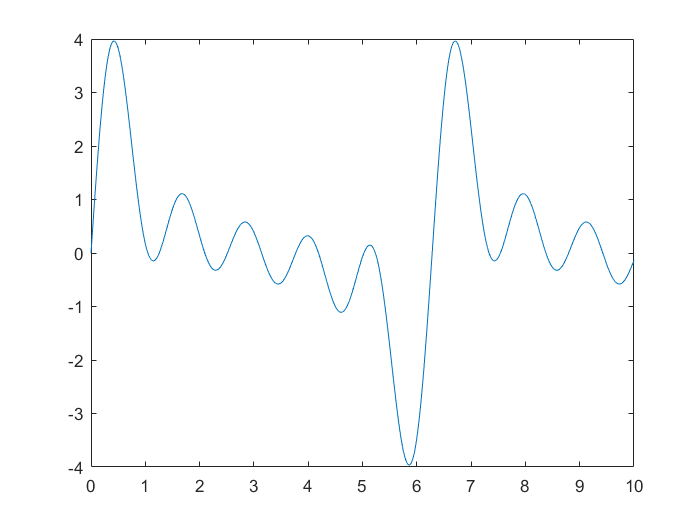
\includegraphics[width=\textwidth]{../figures/summedSinWaves.png}
	\caption{The sum of the first five harmonic sin waves.}
	\label{fig:summedHarmonics}
\end{figure}

Brass instruments are built with the harmonic series in mind.
For example, the tenor trombone has a fundamental pitch of a B$\flat$1, or $58.87$ Hz.
The pitches that can be played on the instrument in first position (i.e. without moving the slide, which would change the fundamental frequency) are those of the harmonic series based on B$\flat$1.
Thus the trombone can theoretically play B$\flat$1, B$\flat$2, F3, B$\flat$3, D4, F4, a very flat G$\sharp$4, B$\flat$4, C5, D5, a very flat E5, F5, and so on.
In practice however, due to the physical demands of the player, any note above B$\flat$4 is uncommon, and any note above D5 is very rare.

When discussing brass instruments, there are some modifications made to the frequencies by shapes of the the bell and mouthpiece of the instrument, but those are beyond the scope of this project.

% Gabriel's Horn

\section{Intervals Between Notes} \label{mathinmusic:intervals}

In order to discuss intervals between notes, we must first choose a tuning system.
The two most common tuning systems are just intonation and equal temperament.

\subsection{Just Intonation} \label{mathinmusic:intervals:just}

Just intonation is based on the concept of perfect intonation, whereby an interval is defined as multiplying a pitch be some rational constant.
Table \ref{table:justintervals} contains the rational ratios for intervals through the first octave.

\begin{table}
	\centering
	\begin{tabular}{c c c}
		Semitones From Base & Ratio & Interval Name\\
		\hline
		0 & $\frac{1}{1}$ & unison\\[4pt]
		1 & $\frac{16}{15}$ & minor second\\[4pt]
		2 & $\frac{9}{8}$ & major second\\[4pt]
		3 & $\frac{6}{5}$ & minor third\\[4pt]
		4 & $\frac{5}{4}$ & major third\\[4pt]
		5 & $\frac{4}{3}$ & perfect fourth\\[4pt]
		6 & $\frac{45}{32}$ & diminished fifth/tritone\\[4pt]
		7 & $\frac{3}{2}$ & perfect fifth\\[4pt]
		8 & $\frac{8}{5}$ & minor sixth\\[4pt]
		9 & $\frac{5}{3}$ & major sixth\\[4pt]
		10 & $\frac{9}{5}$ & minor seventh\\[4pt]
		11 & $\frac{15}{8}$ & major seventh\\[4pt]
		12 & $\frac{2}{1}$ & octave
	\end{tabular}
	\caption{Ratios for intervals under just intonation.}
	\label{table:justintervals}
\end{table}

The just tuning system produces the best sounding intervals and is used to tune intervals by ear.
The downside is that the size of an interval is different than the sum of semi tones to reach the same interval.
For example, the frequency of major third above a given note is $\frac{6}{5}$ that of the given note.
Building that same interval (4 semi tones) by moving up the chromatic scale, however, the ratio is $(\frac{16}{15})^{4} = \frac{65536}{50625} \approx \frac{6.5}{5}$.
This is a significant difference from the ratio for a major third.

\subsection{Equal Temperament} \label{mathinmusic:intervals:equal}

The equal temperament tuning systems breaks the octave into twelve equal parts based on the logarithmic frequency distance from the previous semitone.
That is, each semitone away from the base note is a multiple of a power of the twelfth root of two.
The formula for an interval is $b \times 2^{\frac{x}{12}}$ where $b$ is the frequency of the base note and $x$ is size of the interval in semitones.

The result of this tuning system is that it produces intervals that are close enough to the perfect intervals of just intonation to sound decent for any interval, but do not sound as good as justly tuned intervals.
Modern instruments with fixed pitches such as the piano and guitar use this tuning system.

\subsection{Other Tunning Systems} \label{mathinmusic:intervals:othertuning}


% Get into some group theory?
% prove pitch classes in equally tempered octave form an abelian group with 12 elements + other set and group theory related topics


%!TEX root = ../username.tex
\chapter{A Markov Model for Melody Generation} \label{markov}

\section{Setup of the Model} \label{markov:setup}

In this model, we use two Markov processes: one to determine interval changes between notes to generate pitches, and the other to generate rhythms.
To create the interval transition matrix, we iterate over the source, keeping track of the previous interval at each step, incrementing the matrix at position $a_{i,j}$ for the previous interval $i$ and the current interval $j$.
In our case, the source is a corpus of music by J.S. Bach.
The rhythmic transition matrix is similarly generated.
While iterating over the source to generate the interval transition matrix, we can also build the rhythmic transition matrix.
To do this we keep track of the duration of the previous rhythm at each step and increment the transition matrix at position $b_{k,l}$ for the previous rhythmic duration $k$ and current rhythmic duration $l$.

Because the number of possible intervals and rhythms are theoretically infinite, we do not want to try to store a matrix capable of holding every possible transition.
Instead, we can use a hash table to only store transitions that actually appear in the source.

An example rhythmic transition matrix is given in Figure \ref{fig:rhythmTransitionMatrix}, based on the \textit{Little Fugue in G Minor} by J.S. Bach.

\begin{figure}
	\centering
	\begin{tabular}{c | c c c c c c c c}
		& 0.25 & 0.5 & 0.75 & 1.0 & 1.25 & 1.5 & 2.0 & 2.25\\
		\hline
		0.25 & 606 & 21 & 1 & 2 & 1 & 2 & 0 & 1\\
		0.5 & 23 & 109 & 0 & 7 & 1 & 0 & 0 & 0\\
		0.75 & 1 & 0 & 0 & 0 & 0 & 0 & 0 & 0\\
		1.0 & 1 & 6 & 0 & 3 & 0 & 3 & 2 & 0\\
		1.25 & 2 & 0 & 0 & 0 & 0 & 0 & 0 & 0\\
		1.5 & 0 & 5 & 0 & 0 & 0 & 0 & 0 & 0\\
		2.0 & 0 & 0 & 0 & 2 & 0 & 0 & 0 & 0\\
		2.25 & 1 & 0 & 0 & 0 & 0 & 0 & 0 & 0
	\end{tabular}
	\caption{An example rhythmic transition matrix. A value of $1.0$ indicates a quarter note.}
	\label{fig:rhythmTransitionMatrix}
\end{figure}

\section{Generation} \label{markov:generation}

After the transition matrices are created, the program randomly selects a rhythmic value, based on the probabilities that correspond with the previous note, and a pitch.
The pitch value comes from the interval from the previous note.
The interval is chosen based on the probabilities that correspond with the previous interval.

The program stops generating notes when the stopping criteria are met: the generated melody is at least eight measures, the melody ends at the end of a measure, and the last note is a tonic chord tone.
Because the generated melody could theoretically be infinite, the program terminates generation after one-hundred measures are generated whether or not the stopping criteria are met.

%!TEX root = ../username.tex
\chapter{Genetic Algorithms} \label{ga}

In this project, the melodies generated by the Markov model are used as the initial population for the genetic algorithm.

\section{Fitness Function} \label{ga:fitness}

In several previous papers, the authors discuss the use of interactive fitness functions \cite{papadopoulos_ai_1999, mcvicar_autoguitartab:_2015}.
With this method, a human listens to the melodies and selects the best from each generation to be used as the parents of the next generation.
This method does well at picking the most pleasing music to human ears, but it requires humans to listen to the music, which is slow and can lead to fatigue on the part of the evaluators.

Rather than rely on humans who may become tired, or may slightly vary their definition of good music, we want to use an automated fitness function.
Music from the common practice period of Western music, which lasted from the late Baroque period through the Romantic period (1650-1900), generally followed a complex set of rules regarding harmony, rhythm, and duration.
We could manually define a function that uses some weighted average of each of the many rules, but this approach could be highly error prone and require lots of manual tweaking.

Rather, it is often good enough to approximate a fitness function using what we call a \textit{surrogate model}. % cite a paper on this
Some authors discuss techniques for fitness functions as applied to music \cite{papadopoulos_ai_1999, de_freitas_originality_2011, alfonseca_fitness_2006}.
For example, Alan de Freitas and Frederico Guimaraes use a fitness function that penalizes any note outside of the C Major scale, while George Papadopoulos and Geraint Wiggins use a fitness function that considers several characteristics of the melody, including consecutive intervals, note durations, and contour.
% TODO write about accuracy results from these authors
In this project we use an artificial neural network as the surrogate model.
We expect the neural network to pick up on which rules are the most important, altering its weights accordingly.
Because music has temporal properties, the type of neural network used in this project is a \textit{long short-term memory} (LSTM) network.
An LSTM network is a special type of \textit{recurrent neural network}, where nodes link back to themselves. % TODO write about LSTM networks here

The classification we use is binary: is the chunk of music run through the network similar to the chunks of music used to train the network?
We expect the network might pick up on attributes such as how long a note lasts, what the pitch of a note is, and its relation to the notes around it.
However, we cannot know for certain that the network decides is important before training.

In our corpus of music, the sixteenth note is most commonly the smallest rhythmic value in a piece of music, so we first preprocess the music data by converting all rhythms to consecutive sixteenth notes.
The motivation for this method, rather than trying to encode the rhythm in another way comes from Peter Todd \cite{todd_connectionist_1989}.
We perform additional preprocessing by \textit{one-hot encoding} the pitch class of each note.
This means that each of the twelve pitch classes can be represented as an array of eleven $0$s and one $1$.
For example, C encodes to $[1 \; 0 \; 0 \; 0 \; 0 \; 0 \; 0 \; 0 \; 0 \; 0 \; 0 \; 0]$ and C$\sharp$ encodes to $[0 \; 1 \; 0 \; 0 \; 0 \; 0 \; 0 \; 0 \; 0 \; 0 \; 0 \; 0]$.

Unlike a traditional neural network, an input sample is not entered all at once.
Instead, each note enters the network one at a time.
For this project, we consider four measures of music as input to the neural network.
With our rhythmic encoding of sixteenth notes, this means for each music sample we input $16 * 4 = 64$ notes to the network.
In more general terminology, each note is a \textit{chunk}.
Since each note consists of a single one-hot encoded pitch class, the \textit{chunk size} is $12$.
Somewhat arbitrarily, we use pass the input through $128$ nodes.
The output of the network is a one-hot encode array of two values: is the music sample good enough or not.

During training, in addition to samples of correct music from out corpus, we also feed the network samples of random noise as incorrect examples.

Using this network setup, we were able to achieve up to $93\%$ accuracy when classifying samples from our corpus.

\section{Mutations} \label{ga:mutate}

There are several natural mutations to consider when working with music.
Two common compositional techniques are inversion and retrograde.
Inversion takes a section of music, generally a couple of measures, and inverts all the intervals, so an interval up becomes the same interval down.
Retrograde reverses the order of one or both of the rhythms and pitches of a section of music.
Retrograde and inverse can also be combined, to yield retrograde-inverse.
Typically, the section is inverted, and the new notes are then read backwards, though some composers, such as Igor Stravinsky, reversed the order of the notes first.
See Figure \ref{fig:p-r-i-ri} for an example of inversion, retrograde, and retrograde-inversion.
These techniques are especially common in twelve tone music, which was developed during the early twentieth century by Arnold Schoenberg, though they can also be found in other types of music. % TODO give examples

\begin{figure}
	\centering
	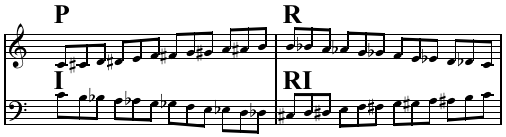
\includegraphics[width=\linewidth]{figures/P-R-I-RI.png} % TODO cite image https://commons.wikimedia.org/wiki/File:P-R-I-RI.png
	\caption{Common  clockwise from the top left: prime (original form), retrograde, inverse, and retrograde-inverse.}
	\label{fig:p-r-i-ri}
\end{figure}

\section{Manipulating Melodies} \label{ga:manip}



%!TEX root = ../username.tex
\chapter{The Software} \label{software}

This chapter discusses the various components of the software used in this project.

All components use music21, a Python library for music developed by MIT, to handle input and output of music notation to and from a Python-native format.
Input files are in MIDI format.

\section{Overview} \label{software:overview}

The data flow for the set of programs used in this project are as follows:
The Markov chain program reads a corpus of music to create its transition matrices.
These Markov chains are then used to produce the initial population for the genetic algorithm.
The genetic algorithm uses a long short term memory artificial neural network as a surrogate fitness function, which was trained with its own music corpus.
The final output from the genetic algorithm then is sent to the harmonization program, which creates other musical voices to accompany the generated melody.
See Figure \ref{fig:softwareoverview} for a visual representation of the broad flow of data.

\begin{figure}[h]
	\centering
	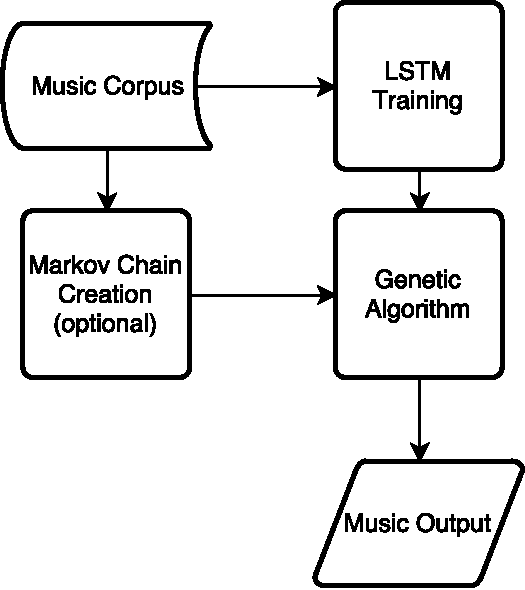
\includegraphics{figures/overview_flowchart.pdf}
	\caption{The flow of data through the software.}
	\label{fig:softwareoverview}
\end{figure}

\section{Markov Melody Generator} \label{software:markov}

In the code repository for this project, the directory \texttt{intervalMarkovChain} contains Python code to generate melodies using Markov chains of arbitrary order.
The theory behind this software component is discussed in Section \ref{bg:markov} and Chapter \ref{markov}.
The software uses two Markov chains to generate a melody, one for the intervals between notes, and the other for rhythms of notes.
See Figure \ref{fig:markovflowchart} for a visual representation of the flow of data through the Markov melody generation.

\begin{figure}[h!]
	\centering
	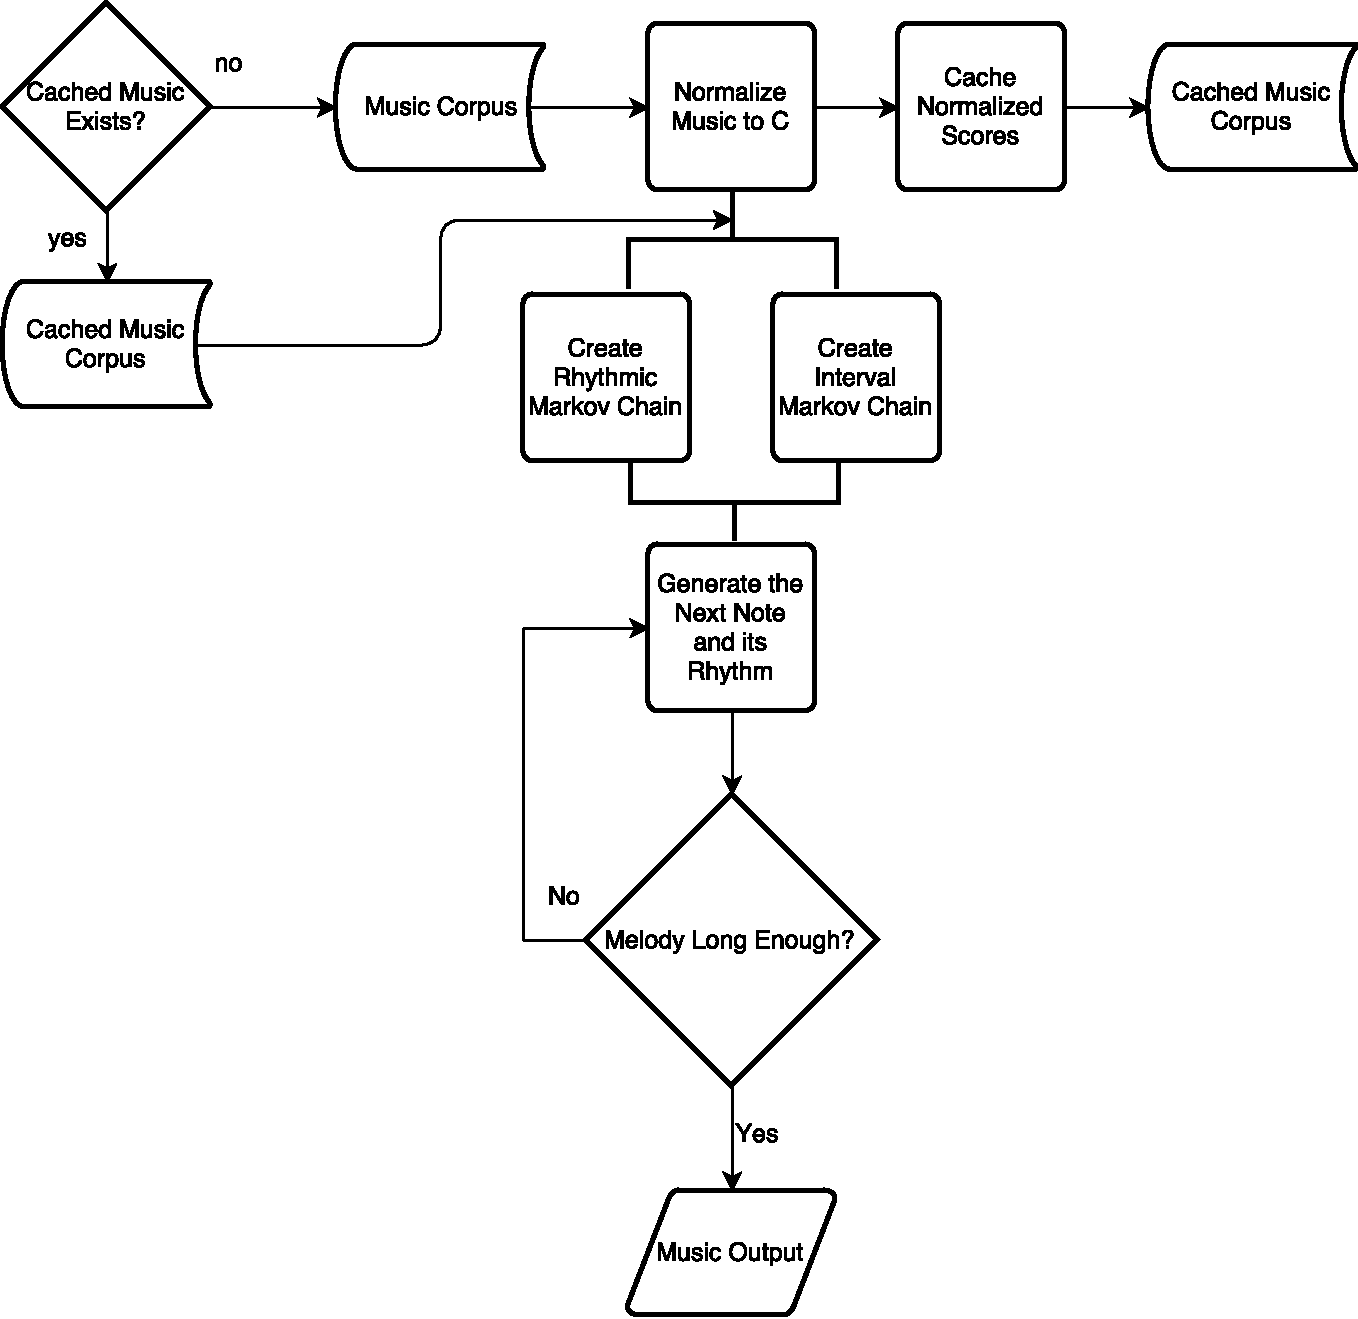
\includegraphics[width=\linewidth]{figures/markov_flowchart.pdf}
	\caption{The flow of data through the creation of a Markov melody.}
	\label{fig:markovflowchart}
\end{figure}

In order to facilitate the creation of Markov chains in a more general way, we create a \texttt{MarkovChain} object, which provides methods to create and use the Markov chain.
When a \texttt{MarkovChain} object is created, it requires an order to use.
By default, the order is $1$.
To create the transition matrix, the function \texttt{create\_transition\_matrix(streams, chainType)} accepts a list of the music21 \texttt{Streams} to use as the training source, as well as what type of Markov chain it should be -- should it calculate transition probabilities for rhythms or for the intervals between notes?

An $n$th order Markov chain is represented using \texttt{defaultdict}s nested $n + 1$ deep.
Two interesting functions in this class are \texttt{arbitrary\_depth\_dict\_get} and \texttt{arbitrary\_depth\_dict\_set}.
These functions allow one to read from and write to \texttt{dict}s of arbitrary depth.
These are necessary to be able to create and use the transition matrices because the order of the Markov chain may not always be the same, so the number of index operators desired cannot be hard-coded.

The function \texttt{arbitrary\_depth\_dict\_get(subscripts, default, nested\_dict)} works by recursively accessing \texttt{nested\_dict} with the first element of \texttt{subscripts} until either \texttt{subscripts} is empty or a key from \texttt{subscripts} does not exist.
In the former case, the function returns the value of \texttt{nested\_dict} specified by \texttt{subscripts}.
In the latter case, the function returns the specified default value.

The function \texttt{arbitrary\_depth\_dict\_set(subscripts, \_dict, val)} works by iterating through the \texttt{subscripts} of \texttt{\_dict}, going a level deeper at each step.
At each level, an empty dictionary is created if one did not already exist at that index.
This function makes use of the fact that the \texttt{dict} data structure in Python can be assigned to a new variable by reference in order to go into the next index.
On the final index, the dictionary is assigned the value at the (possibly nested) index as specified by \texttt{subscripts}.

The \texttt{MarkovChain} class is implemented in \texttt{intervalMarkovChain/markovChain.py}.

In order to create a Markov chain, we need a corpus with which to build it.
Conveniently, music21 provides the ability to read and write a variety of file formats.
In this project, we use MIDI files to store the music we use as a corpus and that we generate.

Because a Markov chain requires some predetermined seed notes to refer to, the first four notes of each generated melody are C, D, E, and D.
These pitches were chosen because the intervals between them (M2 and M-2) will appear in almost any corpus of music at least once.
To keep some rhythmic diversity, the duration for each of these four notes is randomly chosen to be a sixteenth note, eighth note, or quarter note.
The decision to include four seed notes was subjectively made by the author's thoughts that melodies produced using a fourth order interval Markov chain were not sufficiently better than melodies produced using a third order chain to warrant the extra computational cost.
In order to use a Markov chain with an order higher than four, more seed notes must be provided.

Once the interval and rhythm Markov chains are generated and we have our seed notes, we can generate a melody.

The process of reading reading a corpus of music, creating the Markov chains, and generating a melody is implemented in \texttt{intervalMarkovChain/intervalMarkovChain.py}.

\section{Genetic Algorithms} \label{software:ga}

The directory \texttt{geneticAlgorithms} contains Python code to manipulate existing melodies with genetic algorithms to produce better output.
The theory behind this software component is in Section \ref{bg:ga} and Chapter \ref{ga}.

\subsection{Fitness Function} \label{software:ga:fitness}

This program uses an LSTM neural network created using TensorFlow as a surrogate fitness function.
TensorFlow is a machine learning library for Python developed by the Google Brain Team.
The file \texttt{geneticAlgorithms/lstm.py} contains code to convert music data to a form usable by the artificial neural network, train the LSTM neural network on that modified music data, and save the generated model for later use.
See Figure \ref{fig:lstmflowchart} for the flow of data through the creation of the fitness function.

\begin{figure}[h!]
	\centering
	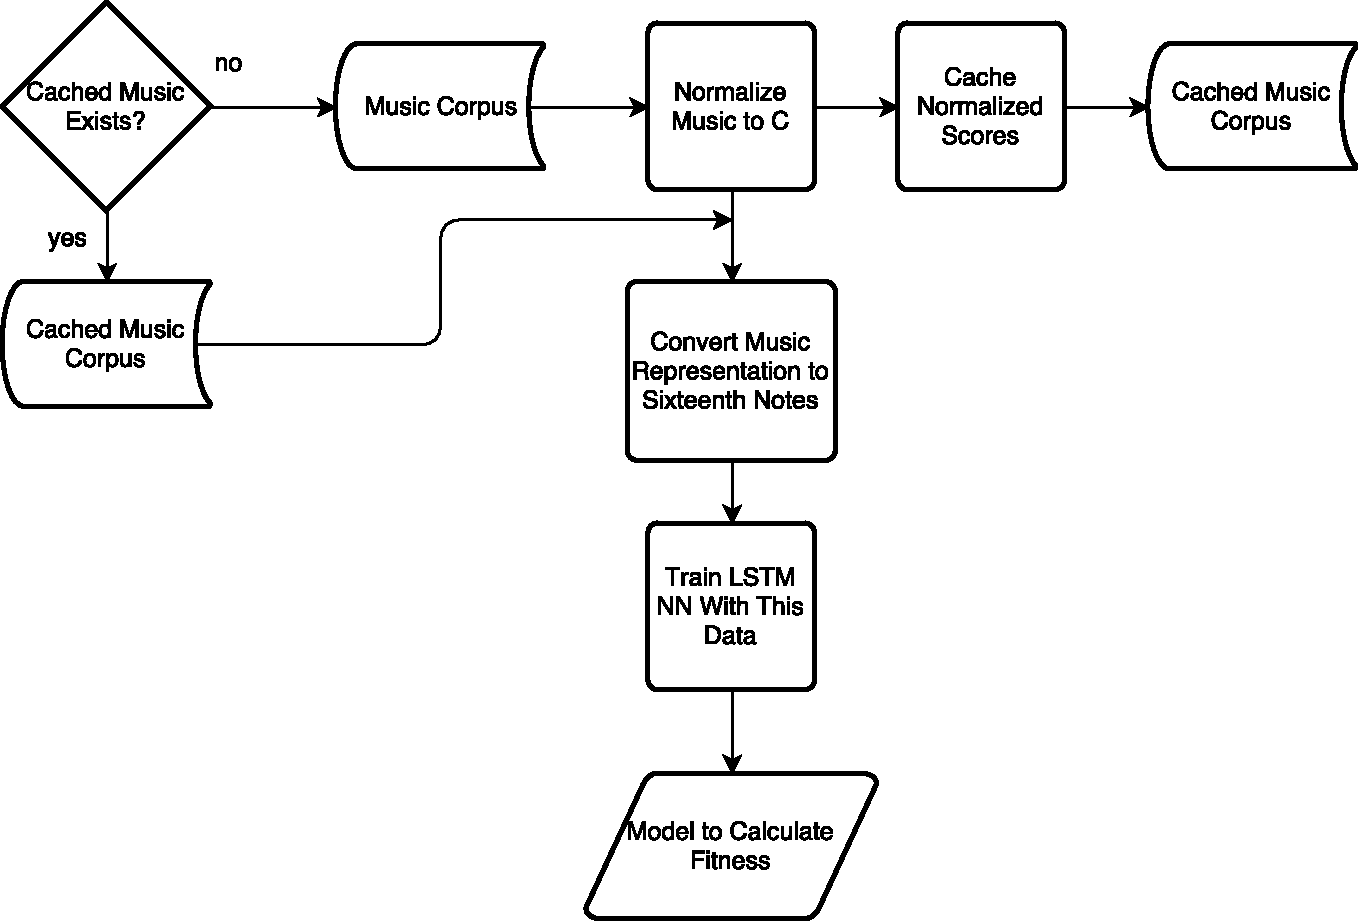
\includegraphics[width=\linewidth]{figures/lstm_flowchart.pdf}
	\caption{The flow of data through the creation of the LSTM neural network to use as the surrogate fitness function.}
	\label{fig:lstmflowchart}
\end{figure}

The first step is to read a corpus of music to train the function on.
If no music corpus is provided, the program uses the collection of Bach chorales that come with music21.
As with the Markov chain module, this module normalizes the melodies to the key of C before training.
This removed the need to take the key a piece is into account.

After the training input is normalized it is converted to a form the artificial neural network will be able to recognize.
We perform some preprocessing by one-hot encoding the pitch of each note.
To limit the range of octaves that can appear in our music, we use the MIDI values for each pitch.
Because the MIDI standard defines values from $0$ to $127$, we can \textit{one-hot encode} the pitch as an array of zeros with a $1$ at the index of the MIDI number we want to represent.
One-hot encoding is a method used in data science to represent categorical data in a numeric format.
Even though the MIDI values are already numeric, we one-hot encode them because the difference of a half step (one MIDI value) can be the distinction between a good melody and a better melody.
Additionally, MIDI values are only ever integer values, so we do not need to represent them as floats.
Importantly, one-hot encoding the MIDI values improves the accuracy of the network.
Now that the good music data is in a form the neural network can recognize, a number of random sequences of sixteenth notes is generated to act as samples of bad samples.
We want the neural network to train on an evenly distributed sampling of good and bad data, so we shuffle the list.

Now the program is ready to create and train the LSTM network.
Unlike a traditional neural network, an input sample is not entered all at once.
Instead, each note enters the network one at a time.
For this project, we consider four measures of 4/4 music as input to the neural network.
With our rhythmic encoding of sixteenth notes, this means for each music sample we input $16 * 4 = 64$ notes to the network.
In more general terminology, each note is a \textit{chunk}.
Since each note consists of a single one-hot encoded pitch, the \textit{chunk size} is $128$.
Somewhat arbitrarily, we pass each input through $256$ neurons in the network.
The output of the network is an array containing two values, which are the network's certainty that the input is or is not a good melody.

To train the model, we run the training data through a function to reshape it to a $N$ x 64 x 128 list, where $N$ is the number of training samples.
$70\%$ of this reshaped data is then fed through the neural network for five epochs.
That is, the data is fed to the network and weights are adjusted five times.
At this point, the accuracy of the model is found by evaluating the remaining $30\%$ of the training data and comparing the output to the actual labels.
If the accuracy is sufficient, the TensorFlow session and the model are returned to be used on new data later.

\subsection{Mutations} \label{software:ga:mutations}

Section \ref{ga:mutate} contains the theoretical background of these mutations.

Because we are working with music data, there are some specific operations we can perform to act as a type of mutation.

The six functions we use to operate on music21 \texttt{stream} objects are \texttt{transpose()}, \texttt{inverse()}, \texttt{retrograde()}, \texttt{retrograde\_inverse()}, \texttt{inverse\_retrograde()}, and \texttt{crossover()}.

\texttt{transpose(stream, interval)} is simply a wrapper for music21's \texttt{Stream.transpose()} method.
It accepts a \texttt{Stream} and an amount to transpose by, measured in semitones.

\texttt{inverse(stream)} returns the inverse of \texttt{stream}.
That is, it takes the inverts the intervals between notes.
For example, the sequence CDE becomes CB$\flat$A$\flat$.

\texttt{retrograde(stream, reverse\_notes, reverse\_rhythms)} returns the retrograde version of \texttt{stream}, with the options to reverse the pitches, the rhythms, or both.

\texttt{retrograde\_inverse(stream)} and \texttt{inverse\_retrograde(stream)} are wrapper functions for \texttt{inverse()} and \texttt{retrograde()}.

\texttt{crossover(parent1, parent2, crossover\_points)} provides the ability to perform crossover of two \texttt{Stream}s.
The function returns two new \texttt{Stream}s.
The first \texttt{Stream} we return is obtained by copying notes from \texttt{parent1} until the first index in \texttt{crossover\_points} is reached, then copying notes from \texttt{parent2} until the second index in \texttt{crossover\_points}, and so on, alternating which parent's notes are copied, until there are no more indices in \texttt{crossover\_points}.
The second returned \texttt{Stream} is obtained similarly, but starts by copying notes from \texttt{parent2}.

These functions are implemented in \texttt{geneticAlgorithms/mutations.py}

\subsection{Evolving Melodies} \label{software:ga:evolving}

The file \texttt{geneticAlgorithms/geneticAlgorithms.py} contains code to carry out the genetic algorithm that takes some initial population of melodies, remixes and mutates them, and eventually produces some more fit output as measured by the fitness function.
It includes uses all of the previously discussed components to achieve this.
See Figure \ref{fig:gaflowchart} for the flow of data through the use of genetic algorithms to generate melodies.

\begin{figure}[h!]
	\centering
	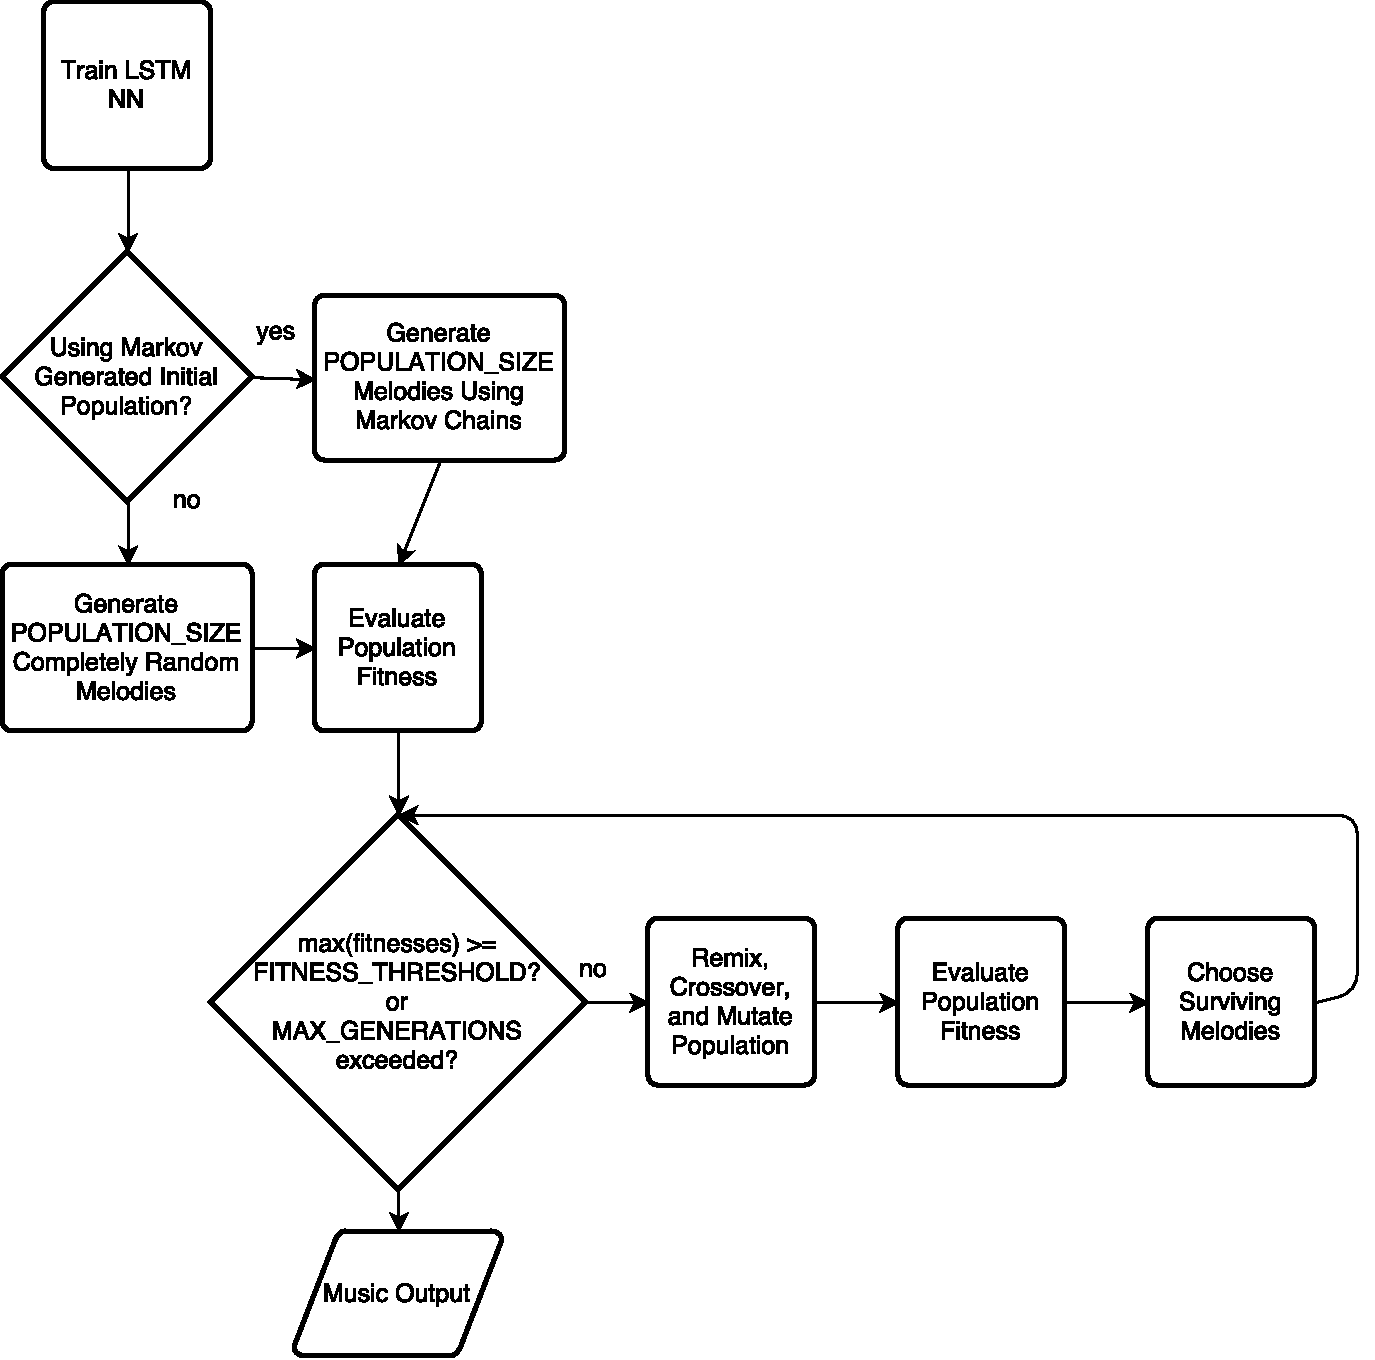
\includegraphics[width=\linewidth]{figures/genetic_algorithm_flowchart.pdf}
	\caption{The flow of data through the use of genetic algorithms to generate melodies.}
	\label{fig:gaflowchart}
\end{figure}

The program starts by creating the fitness function using \texttt{lstm.py}.
Then the initial population is produced.
This can either use \texttt{intervalMarkovChain/intervalMarkovChain.py} to generate the initial population, or use completely random music to accomplish this.
Starting with the Markov chain will generally produce an initial population with a higher fitness, but it will take more time to generate the population.
The fitness values of the initial population are calculated while the initial population is being generated.

At this point the program is ready to enter the main loop.
Its stopping conditions are when a melody has a high enough fitness, or the maximum number of generations has been reached.
Inside the loop, the program uses the \texttt{multiprocess} library to create a pool of workers to remix the population using the functions inside of \texttt{mutations.py}.
% TODO explain why the choice to use multiprocess was made
After this remixing, the loop generates some melodies using crossover, and mutates some of the melodies.
This mutation is to ensure the population does not stagnate.
At this point the loop calculates the fitnesses of the new population, chooses the seed population for the next generation, and goes back to the beginning of the loop.

% \section{Harmonization and Counterpoint}


\section{How to Use the Software} \label{software:howtouse}

\subsection{Markov Melody} \label{software:howtouse:markov}

To produce a melody using the Markov Melody program, call the program \texttt{intervalMarkovChain.py} along with the corpus of music to use, either directly as the MIDI files to use, or as a directory containing MIDI files.
If no corpus is provided, it defaults to any \texttt{.mid} files located in the relative directory \texttt{../corpus}.
From the command line, this might look like

\texttt{python3 intervalMarkovChain.py song1.mid song2.mid}

\noindent when directly specifying the MIDI files to use, or

\texttt{python3 intervalMarkovChain.py}

\noindent to use the default music corpus.
The function \texttt{generate\_melody()} also checks if the parameter \texttt{corpus} is set to \texttt{False}.
In this case that it is \texttt{False}, the function uses the built in music21 collection of Bach chorales.
This option is only available when importing the file from another Python script.


\subsection{Genetic Melody} \label{software:howtouse:ga}

Run \texttt{python3 geneticAlgormithm.py} to generate a set of melodies produced by the genetic algorithm.
The program accepts some optional flags:

\noindent -f, -{}-desired-fitness value 

Sets the fitness required to terminate the program to value

\noindent -s, -{}-population-size value

Sets the size of the population of each generation to value

\noindent -g, -{}-max-generations value

Set the maximum number of generation the program will run to value

\noindent -m

Sets the program to use Markov chains to generate the initial population

For example: To use $5000$ generations with a population of $500$ and a desired fitness of $25$, with the initial population produced using Markov chains, you could use

\texttt{python3 geneticAlgorithm.py -f 25 -g 5000 -s 500 -m}

\noindent or

\texttt{python3 geneticAlgorithm.py --desired-fitness 25 --max-generation 5000 --population-size 500 -m}

%!TEX root = ../username.tex
\chapter{Results and Future Work} \label{results_future}

\section{Results} \label{results}

\subsection{The LSTM Neural Network}

With the neural network setup described in Section \ref{software:ga:fitness}, the network is able to correctly predict whether a set of notes is Bach or not $99\%$ of the time.
This is the same whether it is trained on the Bach cello suites or the chorales provided by music21.
Since the measure of fitness is the difference between the two outputs of the network: how much the network ``thinks'' the sample is and is not Bach music, the possible fitness values range from about $-25$ to $25$, with the occasional melody exceeding this range.
Table \ref{table:fitnesscomp} contains the fitness values for music by Bach, Domenico Scarlatti, and Franz Joseph Haydn.
Two different versions of the fitness function were used, one trained on music21's Bach chorales, and the other on Bach cello suites.
As expected, the fast paced violin sonata by Haydn and the piano exercise by Scarlatti performed much better when using the fitness function trained with the cello suites, which are themselves fast paced pieces of music.

% TODO include figures of the tested music

\begin{table}
	\centering
	\begin{tabular}{c | c c}
		Piece & Fitness (Chorales) & Fitness (Cello Suites) \\
		\hline
		J.S. Bach Cello Suite 1, Mvmt. 1 & $-18.3$ & $12.7$ \\
		J.S. Bach Little Fugue in G Minor & $15.0$ & $11.7$ \\
		Domenico Scarlatti & $4.3$ & $13.6$ \\
		Haydn Violin Sonata & $-10.7$ & $15$
	\end{tabular}
	\caption{Fitness values of music by various authors using models trained with music21's Bach chorales and Bach's cello suites}
	\label{table:fitnesscomp}
\end{table}

As expected, the faster paced music of Haydn, Scarlatti, and Bach's Cello Suite performed better when the neural network was trained using the fast paced Cello Suites, as compared with the slower Bach chorales.

\subsection{Markov Chains vs Random Notes}
Although the initial population's fitness is generally greater when using Markov chains create the melodies, the use of the genetic algorithm quickly negates that difference within a few generations.
There exists the possibility that the fitness of the randomly seeded population to even surpass the fitness of the Markov chain seeded population.
Since the time to generate the initial population using Markov chains is considerable, compared to using list comprehension to create random notes, the Markov chain melodies should be relegated to generating one off melodies.
% TODO insert figures showing fitness over time for random vs Markov start

\subsection{The Music and Its Uses}

\begin{figure}[h]
	\centering
	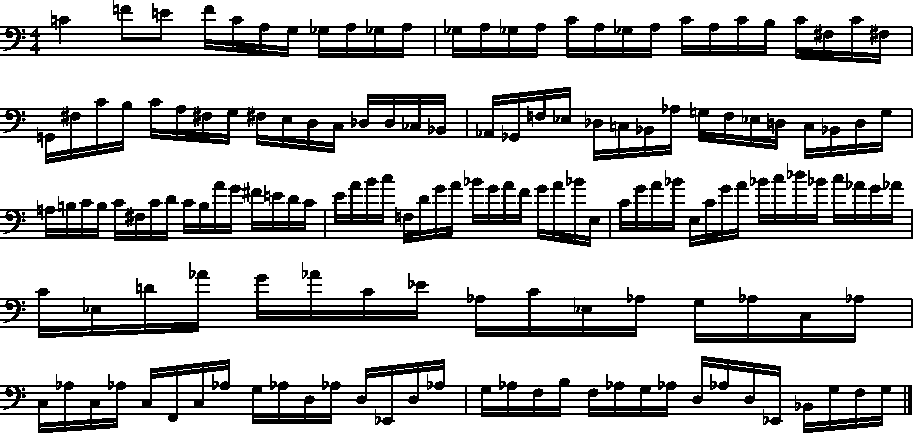
\includegraphics[width=\linewidth]{figures/markov_melody_1.pdf}
	\caption{A melody generated by Markov chains.}
	\label{fig:music:markov1}
\end{figure}

\begin{figure}[h]
	\centering
	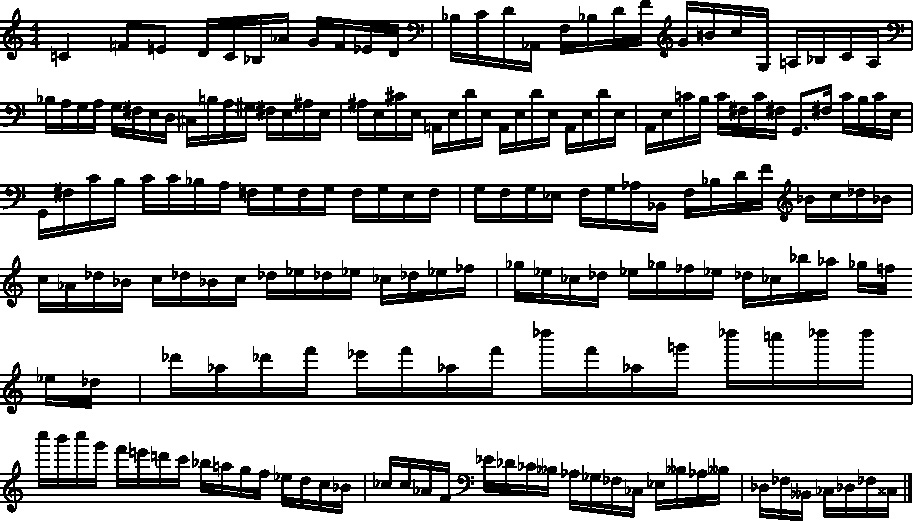
\includegraphics[width=\linewidth]{figures/markov_melody_2.pdf}
	\caption{A melody generated by Markov chains.}
	\label{fig:music:markov2}
\end{figure}

Figures \ref{fig:music:markov1} and \ref{fig:music:markov2} show two melodies generated using Markov chains.
They were generated using a third order Markov chain for the intervals between notes and a second order Markov chain for the rhythms.
Of particular interest, the second measure of the second line of Figure \ref{fig:music:markov2} contains a figure repeated three times.
Additionally, the first measure of the last line of that particular melody contains a perfect run down the B$\flat$ Major scale (from B$\flat$5 to B$\flat$4) in its last two beats.
With the exception of the $E6$ in the second beat of this measure not being an E$\flat$, it is almost a perfect run down the scale starting on G6 and ending on B$\flat$4.

% TODO include figures of randMarkov melodies  (3 & 4 on desktop)

\begin{figure}[h]
	\centering
	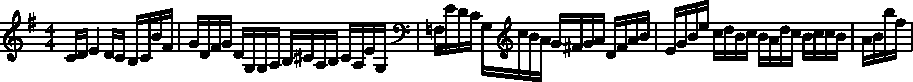
\includegraphics[width=\linewidth]{figures/genetic_melody_1.pdf}
	\caption{A melody generated with the genetic algorithm.}
	\label{fig:music:genetic}
\end{figure}

The melody is Figure \ref{fig:music:genetic} was generated using the genetic algorithm with the surrogate fitness function trained using the chorales from music21's built in corpus of Bach music and an initial population of randomly generated melodies.
Of particular interest in the melody is the set of arpeggiations in the third and fourth measures.
Without explicitly telling the algorithm anything about arpeggiating or repeating ideas in slightly differing ways, it picked up that this makes for good (Bach-like) music.

\begin{figure}[h]
	\centering
	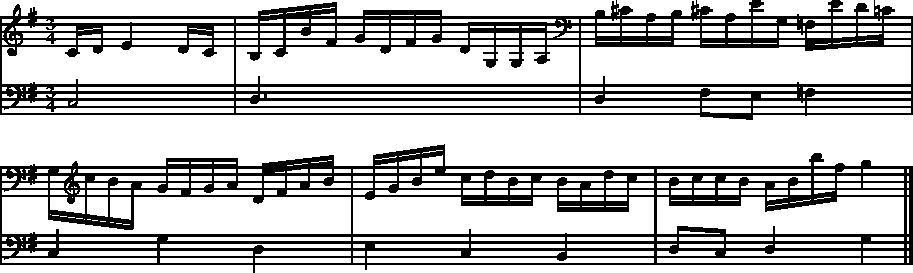
\includegraphics[width=\linewidth]{figures/genetic_melody_1_harmonized.pdf}
	\caption{The melody in Figure \ref{fig:music:genetic} with a bass line written by the author.}
	\label{fig:music:geneticHarmonized}
\end{figure}

Figure \ref{fig:music:geneticHarmonized} showcases one of the potential use cases for the melody generation: compositional inspiration.
The author added a simple bass line to the melody from Figure \ref{fig:music:genetic}, as well as added a more satisfying ending.
% TODO mention work using this melody in Music Tech?

An application of this project is to provide inspiration for the composer.
See Figure \ref{fig:music:geneticHarmonized} for an example where the author used the melody from Figure \ref{fig:music:genetic} and added a bass line.
The generated melodies could also be chained together to create longer compositions, or have their rhythms increased by some multiple to have more than a snippet of music.

The ambitious musician might use these melodies to practice their sight reading; it is extremely unlikely that a melody produced by wither the Markov chains of genetic algorithm has even been written before, let alone seen by a particular musician.
Therefore, these melodies could provide a great opportunity to practice reading music seen for the first time.

\section{Future Work} \label{future}

The work in this project could be expanded by writing code to generate counterpoint or harmonizations of the melodies created using the existing Markov and genetic processes.
One possible method to do this might involve simply using music21's ability to create a \textit{Roman numeral analysis} (RNA) of a piece to determine which chords to use.
Then, the software could fill in the bass, tenor, and alto parts with notes that fit the RNA.
This would likely create very simple, possibly boring, harmonies that may not follow all the voice leading rules of Western music, but it would create \textit{a} complete harmonization.

Many authors have written about the topic of automatic harmonization.
Interestingly, much of the research of this topic focuses on using genetic algorithms to accomplish the task.
William Schottstaedt \cite{schottstdaet_automatic_1989}, defines a genetic algorithm to generate multi-voice music that follows the rules of the Common Practice era.
Somnuk Phon-Amnuaisuk and Geraint A. Wiggins \cite{phon-amnuaisuk_four-part_1999} use genetic algorithms to harmonize preexisting soprano parts.
Andres Acevedo \cite{acevedo_fugue_2004} uses genetic algorithms to write counterpoint in a fugue setting.
A fugue is a music writing technique in which an initial theme is introduced in one part, which is imitated in other parts and repeated throughout the piece.
There are many other examples of using genetic algorithms to solve harmonization and counterpoint; these are just a small sample of the approaches explored.

Other approaches than using genetic algorithms exist for creating pleasing counterpoint.
For example, David Cope discusses a rule based approach to writing counterpoint \cite{cope_computers_1991}.
In this method, a set of rules about how to compose is provided to the program, rather than the program learning from the music on which it is based.
In another approach, Kamil Adiloglu and Ferda Alpaslan \cite{adiloglu_machine_2007} use a feed forward neural network to accept a single voice melody and produce a second voice to complement the first one.

Along with adding counterpoint or harmony generation, other machine learning approaches, one might take different approaches to produce melodies.
For example, Chun-Chi Chen and Risto Miikkulainen \cite{chen_creating_2001} combine neural networks and genetic algorithms by using an evolutionary algorithm to find neural networks that produce good melodies.

% By expanding this project, its use could go beyond merely providing musical inspiration to the composer; it could create entire works, complete with a melody, bass line, and parts in between.


%%%%%%%%%%%%%%%%%%%%%%%%%%%%%%%%%%%%%%%%%%%%%%%%%%%%%%%
%
%  This section starts the back matter. The back matter includes appendices, indicies, and the
%  bibliography
%
%%%%%%%%%%%%%%%%%%%%%%%%%%%%%%%%%%%%%%%%%%%%%%%%%%%%%%%

\backmatter

% \input{appendices/math}

%%%%%%%%%%%%%%%%%%%%%%%%%%%%%%%%%%%%%%%%%%%%%%%%%%%%%%%
%
%  This section would be used if you are not using BibTeX. Look at Kopka and Daly for how to
%  format a bibliography manually as well as how to use BibTeX.
%
%%%%%%%%%%%%%%%%%%%%%%%%%%%%%%%%%%%%%%%%%%%%%%%%%%%%%%%

%\begin{thebibliography}{99}
%\bibitem{}
%\bibitem{}
%\end{thebibliography}

%%%%%%%%%%%%%%%%%%%%%%%%%%%%%%%%%%%%%%%%%%%%%%%%%%%%%%%
%
%  We used BibTeX to generate a Bibliography. I would recommend this method. However, it is
%  not required.
%
%%%%%%%%%%%%%%%%%%%%%%%%%%%%%%%%%%%%%%%%%%%%%%%%%%%%%%%

\renewcommand\bibname{References} % changes the name of the Bibliography

\nocite{*} % This command forces all the bibliography references to be printed -- not just 
              % those that were explicitly cited in the text.  If you comment this out, the bibliography
              % will only include cited references.
\ifthenelse{\boolean{woosterchicago}}{
\bibliographystyle{woosterchicago}}{\ifthenelse{\boolean{achemso}}{
\bibliographystyle{achemso}}{\bibliographystyle{plainnat}}}
% if you have used the woosterchicago class option then your references and citations will be in Chicago format. If you have used the achemso class option then your references and citations will be in the American Chemical Society format. If you do not specify a citation format then the default Wooster format will be used.
\bibliography{references} % load our Bibliography file

%%%%%%%%%%%%%%%%%%%%%%%%%%%%%%%%%%%%%%%%%%%%%%%%%%%%%%%
%
%                                                                Index
%
%  Uncomment the lines below to include an index. To get an index you must put 
%  \index{index text} after any words that you want to appear in the index.
%  Subentries are entered as \index{index text!subentry text}. You must also run the
%  makeindex program to generate the index files that LaTeX uses. The PCs are set to run
%  makeindex automatically.
%
%%%%%%%%%%%%%%%%%%%%%%%%%%%%%%%%%%%%%%%%%%%%%%%%%%%%%%%

%\ifthenelse{\boolean{index}}{
%\cleardoublepage
%\phantomsection
%\addcontentsline{toc}{chapter}{Index}
%\printindex}{}

%%%%%%%%%%%%%%%%%%%%%%%%%%%%%%%%%%%%%%%%%%%%%%%%%%%%%%%
%
%                                                                Colophon
%
%  A Colophon is a section of a printed document that acknowledges the designers and printers of the work.
% The colophon also includes information about the fonts and paper used in the printing. It is not required 
% for your IS and can be commented out.
%
%%%%%%%%%%%%%%%%%%%%%%%%%%%%%%%%%%%%%%%%%%%%%%%%%%%%%%%

%\ifthenelse{\boolean{colophon}}{
%\begin{colophon}
%This Independent Study was designed by Dr. Jon Breitenbucher.\newline
%It was edited and set into type in Wooster, Ohio,\newline
%using the \ifthenelse{\boolean{xetex}}{\XeTeX\ typesetting system designed by Jonathan Kew}{\LaTeX\ typesetting system designed by Leslie Lamport}\newline
%and based on the original \TeX\ system of Donald Knuth.\newline
%It was printed and bound by Office Services at The College of Wooster.
%
%The text face is Adobe Garamond Pro, designed by Robert Slimbach.\newline
%This is the Opentype version distributed by Adobe Systems\newline
%and purchased as part of the Adobe Type Classics for Learning.
%
%The paper is standard laser copier paper and not of archival quality.
%\end{colophon}}{}
\clearpage\thispagestyle{empty}\null\clearpage
\end{document}